\documentclass[a4paper]{article}\usepackage[]{graphicx}\usepackage[]{color}
%% maxwidth is the original width if it is less than linewidth
%% otherwise use linewidth (to make sure the graphics do not exceed the margin)
\makeatletter
\def\maxwidth{ %
  \ifdim\Gin@nat@width>\linewidth
    \linewidth
  \else
    \Gin@nat@width
  \fi
}
\makeatother

\definecolor{fgcolor}{rgb}{0.345, 0.345, 0.345}
\newcommand{\hlnum}[1]{\textcolor[rgb]{0.686,0.059,0.569}{#1}}%
\newcommand{\hlstr}[1]{\textcolor[rgb]{0.192,0.494,0.8}{#1}}%
\newcommand{\hlcom}[1]{\textcolor[rgb]{0.678,0.584,0.686}{\textit{#1}}}%
\newcommand{\hlopt}[1]{\textcolor[rgb]{0,0,0}{#1}}%
\newcommand{\hlstd}[1]{\textcolor[rgb]{0.345,0.345,0.345}{#1}}%
\newcommand{\hlkwa}[1]{\textcolor[rgb]{0.161,0.373,0.58}{\textbf{#1}}}%
\newcommand{\hlkwb}[1]{\textcolor[rgb]{0.69,0.353,0.396}{#1}}%
\newcommand{\hlkwc}[1]{\textcolor[rgb]{0.333,0.667,0.333}{#1}}%
\newcommand{\hlkwd}[1]{\textcolor[rgb]{0.737,0.353,0.396}{\textbf{#1}}}%
\let\hlipl\hlkwb

\usepackage{framed}
\makeatletter
\newenvironment{kframe}{%
 \def\at@end@of@kframe{}%
 \ifinner\ifhmode%
  \def\at@end@of@kframe{\end{minipage}}%
  \begin{minipage}{\columnwidth}%
 \fi\fi%
 \def\FrameCommand##1{\hskip\@totalleftmargin \hskip-\fboxsep
 \colorbox{shadecolor}{##1}\hskip-\fboxsep
     % There is no \\@totalrightmargin, so:
     \hskip-\linewidth \hskip-\@totalleftmargin \hskip\columnwidth}%
 \MakeFramed {\advance\hsize-\width
   \@totalleftmargin\z@ \linewidth\hsize
   \@setminipage}}%
 {\par\unskip\endMakeFramed%
 \at@end@of@kframe}
\makeatother

\definecolor{shadecolor}{rgb}{.97, .97, .97}
\definecolor{messagecolor}{rgb}{0, 0, 0}
\definecolor{warningcolor}{rgb}{1, 0, 1}
\definecolor{errorcolor}{rgb}{1, 0, 0}
\newenvironment{knitrout}{}{} % an empty environment to be redefined in TeX

\usepackage{alltt}

\usepackage{hyperref}
\usepackage{graphicx}
\usepackage{underscore}

\newcommand{\Rfunction}[1]{{\texttt{#1}}}
\newcommand{\Rmethod}[1]{{\texttt{#1}}}
\newcommand{\R}{\textbf{\emph{R\,}}}

\newcommand{\Robject}[1]{{\texttt{#1}}}
\newcommand{\Rpackage}[1]{{\textit{#1}}}
\newcommand{\Rclass}[1]{{\textit{#1}}}


\newcommand{\classdef}[1]{%
  {\em #1}
}

\pagestyle{plain}

\title{Introduction to Bioconductor class \texttt{ExpressionSet}}
\author{Alex Sanchez}



\IfFileExists{upquote.sty}{\usepackage{upquote}}{}
\begin{document}

\maketitle

\thispagestyle{empty}

\tableofcontents

\section{Introduction. Working with Omics data}

Omics data are not only high throughput, what means we require big dta matrices to store raw data. They are also complex and, besides numerical data, they often require additional information such as covariates, annotations or technical information required for preprocessing the data.

In this lab we introduce the \texttt{ExpressionSet} class as an option for managing all these pieces of information simultaneously, which not only simplifies the process but also prevents mistakes derived from lack of consistency between the parts.

We start illustrating with a toy example what would be a ``standard approach'' to managing an omics dataset. Next we introduce the OOP paradigm and a Bioconductor class that allows encapsulating all the informations together and show how it facilitates the process of storing, managing and analyzing omics data.

\subsection{A toy dataset}

For the purpose of this lab we are going to simulate a toy (fake) dataset that consists of the following:
\begin{description}
\item[Expression values] A matrix of 30 rows and 10 columns containing expression values from a gene expression experiment. Matrix column names are sample identifiers
\item[Covariates] A table of ten rows and four columns containing the sample identifiers, the treatment groups and the age and sex of individuals.
\item{Genes} Information about the features contained in the data. May be the gene names, the probeset identifiers etc. Usually stored in a character vector but may also be a table with distinct annotations per feature.
\item[Information about the experiment] Additional information about the study, such as the authors and their contact details or the title and url of the study that originated them.
\end{description}

\begin{knitrout}
\definecolor{shadecolor}{rgb}{0.969, 0.969, 0.969}\color{fgcolor}\begin{kframe}
\begin{alltt}
\hlstd{expressionValues} \hlkwb{<-} \hlkwd{matrix} \hlstd{(}\hlkwd{rnorm} \hlstd{(}\hlnum{300}\hlstd{),} \hlkwc{nrow}\hlstd{=}\hlnum{30}\hlstd{)}
\hlkwd{colnames}\hlstd{(expressionValues)} \hlkwb{<-} \hlkwd{paste0}\hlstd{(}\hlstr{"sample"}\hlstd{,}\hlnum{1}\hlopt{:}\hlnum{10}\hlstd{)}
\hlkwd{head}\hlstd{(expressionValues)}
\end{alltt}
\begin{verbatim}
##          sample1     sample2     sample3    sample4    sample5    sample6
## [1,]  0.34369662  0.78823091 -1.44177165 -0.7266339 0.39270155 -0.5717577
## [2,]  0.08211110  0.20145515 -0.17826983 -0.1991470 0.04898769  0.3044198
## [3,]  1.26830733  0.85615633 -0.31455846 -1.1569649 0.26111225  0.3779398
## [4,] -1.18745479 -0.06958821  0.97127133 -0.1442893 2.54421016  0.7096269
## [5,]  0.09012818  2.80657915  1.33035629 -0.2506080 1.01565316  0.5385987
## [6,] -1.36883880 -0.09024312 -0.02837428  1.6989627 0.97407279  0.7977909
##          sample7    sample8    sample9   sample10
## [1,]  0.74944697  0.5271380  0.5113672  0.3994993
## [2,]  2.09004745  0.7277956 -0.4489498  0.8279574
## [3,]  1.23031729  0.0606610 -0.8256985  0.6623504
## [4,] -1.22395185  1.3703740 -0.4430325 -1.2101024
## [5,] -0.05406224 -1.8356286  0.8337383  0.1933899
## [6,] -1.71415093 -1.8292895  1.6613754  0.2356994
\end{verbatim}
\end{kframe}
\end{knitrout}

\begin{knitrout}
\definecolor{shadecolor}{rgb}{0.969, 0.969, 0.969}\color{fgcolor}\begin{kframe}
\begin{alltt}
\hlstd{targets} \hlkwb{<-} \hlkwd{data.frame}\hlstd{(}\hlkwc{sampleNames} \hlstd{=} \hlkwd{paste0}\hlstd{(}\hlstr{"sample"}\hlstd{,}\hlnum{1}\hlopt{:}\hlnum{10}\hlstd{),} \hlkwc{group}\hlstd{=}\hlkwd{c}\hlstd{(}\hlkwd{paste0}\hlstd{(}\hlstr{"CTL"}\hlstd{,}\hlnum{1}\hlopt{:}\hlnum{5}\hlstd{),}\hlkwd{paste0}\hlstd{(}\hlstr{"TR"}\hlstd{,}\hlnum{1}\hlopt{:}\hlnum{5}\hlstd{)),}\hlkwc{age} \hlstd{=} \hlkwd{rpois}\hlstd{(}\hlnum{10}\hlstd{,} \hlnum{30}\hlstd{),} \hlkwc{sex}\hlstd{=}\hlkwd{as.factor}\hlstd{(}\hlkwd{sample}\hlstd{(}\hlkwd{c}\hlstd{(}\hlstr{"Male"}\hlstd{,} \hlstr{"Female"}\hlstd{),}\hlnum{10}\hlstd{,}\hlkwc{replace}\hlstd{=}\hlnum{TRUE}\hlstd{)))}
\hlkwd{head}\hlstd{(targets,} \hlkwc{n}\hlstd{=}\hlnum{10}\hlstd{)}
\end{alltt}
\begin{verbatim}
##    sampleNames group age    sex
## 1      sample1  CTL1  34 Female
## 2      sample2  CTL2  32   Male
## 3      sample3  CTL3  26 Female
## 4      sample4  CTL4  30   Male
## 5      sample5  CTL5  36 Female
## 6      sample6   TR1  30   Male
## 7      sample7   TR2  27   Male
## 8      sample8   TR3  25 Female
## 9      sample9   TR4  29   Male
## 10    sample10   TR5  30   Male
\end{verbatim}
\end{kframe}
\end{knitrout}

\begin{knitrout}
\definecolor{shadecolor}{rgb}{0.969, 0.969, 0.969}\color{fgcolor}\begin{kframe}
\begin{alltt}
\hlstd{myGenes} \hlkwb{<-}  \hlkwd{paste0}\hlstd{(}\hlstr{"gene"}\hlstd{,}\hlnum{1}\hlopt{:}\hlnum{30}\hlstd{)}
\end{alltt}
\end{kframe}
\end{knitrout}

\begin{knitrout}
\definecolor{shadecolor}{rgb}{0.969, 0.969, 0.969}\color{fgcolor}\begin{kframe}
\begin{alltt}
\hlstd{myInfo}\hlkwb{=}\hlkwd{list}\hlstd{(}\hlkwc{myName}\hlstd{=}\hlstr{"Alex Sanchez"}\hlstd{,} \hlkwc{myLab}\hlstd{=}\hlstr{"Bioinformatics Lab"}\hlstd{,}
          \hlkwc{myContact}\hlstd{=}\hlstr{"alex@somemail.com"}\hlstd{,} \hlkwc{myTitle}\hlstd{=}\hlstr{"Practical Exercise on ExpressionSets"}\hlstd{)}
\hlkwd{show}\hlstd{(myInfo)}
\end{alltt}
\begin{verbatim}
## $myName
## [1] "Alex Sanchez"
## 
## $myLab
## [1] "Bioinformatics Lab"
## 
## $myContact
## [1] "alex@somemail.com"
## 
## $myTitle
## [1] "Practical Exercise on ExpressionSets"
\end{verbatim}
\end{kframe}
\end{knitrout}

Having data stored in this way is usually enough for most of the analyes we may want to do.
The only unconvenient comes from the fact that the information about the same individuals is in separate R objects so that, for certain applications, we will have to access several objects and \emph{assume they are well related}.

For example if we want to make a principal components analysis and plot the groups by treatment we need to use both ``expressionValues" and ``targets."

\begin{knitrout}
\definecolor{shadecolor}{rgb}{0.969, 0.969, 0.969}\color{fgcolor}\begin{kframe}
\begin{alltt}
\hlstd{pcs} \hlkwb{<-} \hlkwd{prcomp}\hlstd{(expressionValues)}
\hlkwd{names}\hlstd{(pcs)}
\end{alltt}
\begin{verbatim}
## [1] "sdev"     "rotation" "center"   "scale"    "x"
\end{verbatim}
\begin{alltt}
\hlkwd{barplot}\hlstd{(pcs}\hlopt{$}\hlstd{sdev)}
\end{alltt}
\end{kframe}
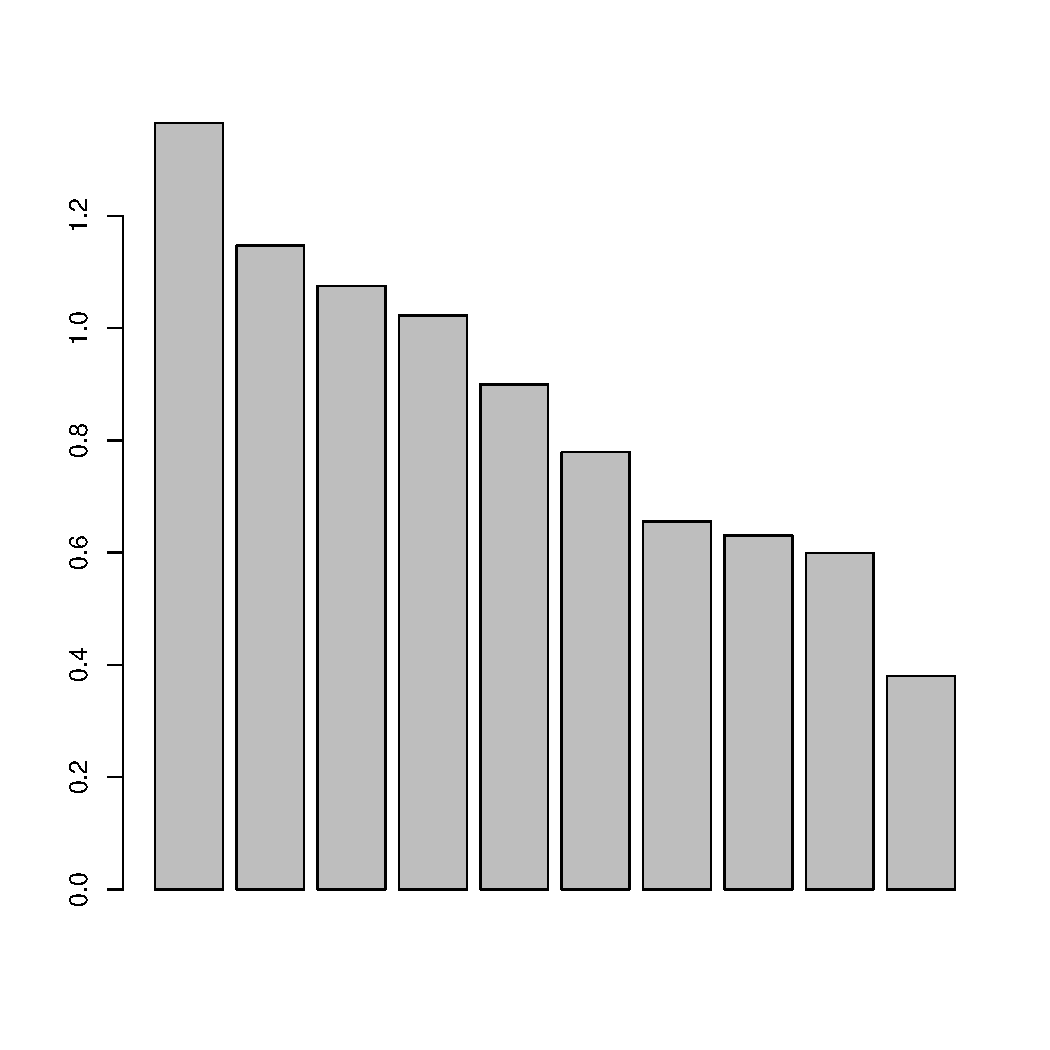
\includegraphics[width=\maxwidth]{figure/unnamed-chunk-2-1} 
\begin{kframe}\begin{alltt}
\hlkwd{plot}\hlstd{(pcs}\hlopt{$}\hlstd{rotation[,}\hlnum{1}\hlstd{], pcs}\hlopt{$}\hlstd{rotation[,}\hlnum{2}\hlstd{],} \hlkwc{col}\hlstd{=targets}\hlopt{$}\hlstd{group,} \hlkwc{main}\hlstd{=}\hlstr{"Representation of first two principal components"}\hlstd{)}
\hlkwd{text}\hlstd{(pcs}\hlopt{$}\hlstd{rotation[,}\hlnum{1}\hlstd{], pcs}\hlopt{$}\hlstd{rotation[,}\hlnum{2}\hlstd{],targets}\hlopt{$}\hlstd{sex)}
\end{alltt}
\end{kframe}
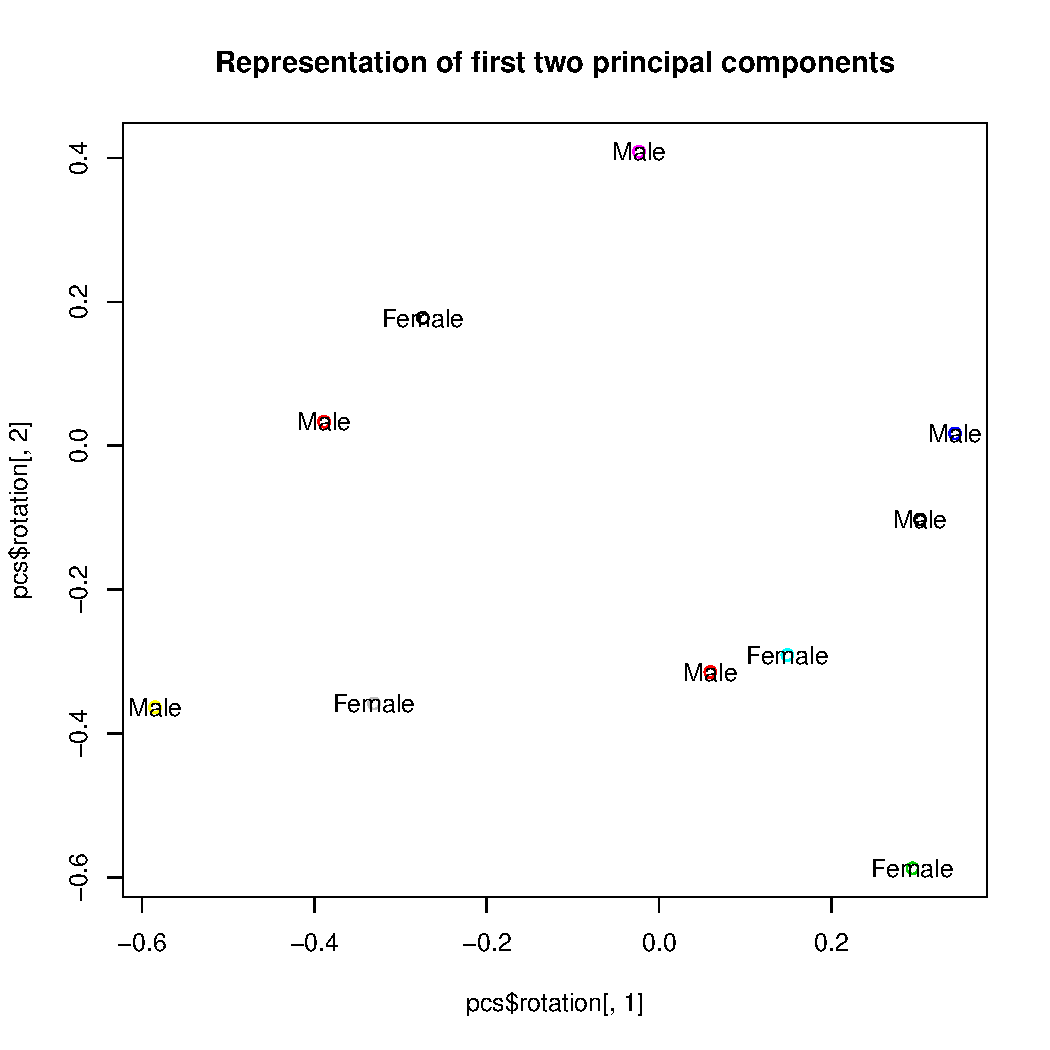
\includegraphics[width=\maxwidth]{figure/unnamed-chunk-2-2} 

\end{knitrout}

Or, if we sort the genes from most to least variable and whant to see which are the top variable genes. We need to use both objects ``expressionValues" and ``myGenes" assuming they are well linked:

\begin{knitrout}
\definecolor{shadecolor}{rgb}{0.969, 0.969, 0.969}\color{fgcolor}\begin{kframe}
\begin{alltt}
\hlstd{variab} \hlkwb{<-} \hlkwd{apply}\hlstd{(expressionValues,} \hlnum{1}\hlstd{, sd)}
\hlstd{orderedGenes} \hlkwb{<-} \hlstd{myGenes[}\hlkwd{order}\hlstd{(variab,} \hlkwc{decreasing}\hlstd{=}\hlnum{TRUE}\hlstd{)]}
\hlkwd{head}\hlstd{(variab[}\hlkwd{order}\hlstd{(variab,} \hlkwc{decreasing}\hlstd{=}\hlnum{TRUE}\hlstd{)])}
\end{alltt}
\begin{verbatim}
## [1] 1.309937 1.256927 1.200237 1.188556 1.139880 1.122894
\end{verbatim}
\begin{alltt}
\hlkwd{head}\hlstd{(orderedGenes)}
\end{alltt}
\begin{verbatim}
## [1] "gene6"  "gene4"  "gene5"  "gene13" "gene17" "gene18"
\end{verbatim}
\end{kframe}
\end{knitrout}

Imagine we are informed that individual has to be removed. We have to do it in ``expressionValues'' and ``targets''.

\begin{knitrout}
\definecolor{shadecolor}{rgb}{0.969, 0.969, 0.969}\color{fgcolor}\begin{kframe}
\begin{alltt}
\hlstd{newExpress}\hlkwb{<-} \hlstd{expressionValues[,}\hlopt{-}\hlnum{9}\hlstd{]}
\hlstd{newTargets} \hlkwb{<-} \hlstd{targets[}\hlopt{-}\hlnum{9}\hlstd{,]}
\hlstd{wrongNewTargets} \hlkwb{<-} \hlstd{targets [}\hlopt{-}\hlnum{10}\hlstd{,]}
\end{alltt}
\end{kframe}
\end{knitrout}
                                                                                                            It is relatively easy to make an unnoticeable mistake in removing unrelated values from the data matrix and the targets table. If instead of removing individual 9 we remove individual 10 it may be  difficult to realize what has happened unless it causes a clear unconsistency!

Next section introduces a data structure that allows to encapsulate all these informations together ensuring that the links assumed are true.

\section{Bioconductor classes for omics data}

\subsection{The OOP paradigm}

Object-oriented design provides a convenient way to represent data structures and actions performed on them.
\begin{itemize}
  \item A \emph{class} can be tought of as a template, a description of what constitutes each instance of the class.
  \item An \emph{instance} of a class is a realization of what describes the class.
  \item Attributes of a class are data components, and methods of a class are functions, or actions the instance/class is capable of.
\end{itemize}

The {\it R} language has several implementations of the OO paradigm but, in spite of its success in other languages, it is relatively minoritary.


\subsection{Bioconductor Classes}

One case where OOP has succeeded in R or, at least, is more used than in others is in the Bioconductor Project (\url{http://bioconductor.org}). In Bioconductor we have to deal with complex data structures such as the results of a microarray experiment, a genome and its annotation or a complex multi-omics dataset. These are situations where using OOP to create classes to manage those complex types of data is clearly appropriate.

\subsection{The Biobase package}

The \Rpackage{Biobase} package implements one of the best known Bioconductor classes: \texttt{ExpressionSet}. It was originally intended to contain microarray data and information on the study that generated them and it has become a standard for similar data structures.

\begin{knitrout}
\definecolor{shadecolor}{rgb}{0.969, 0.969, 0.969}\color{fgcolor}\begin{kframe}
\begin{alltt}
\hlkwd{require}\hlstd{(Biobase)}
\end{alltt}
\end{kframe}
\end{knitrout}

Figure \ref{fig:ExpressionSet}~ shows the structure of this class. It is essentially a \emph{container} that has distinct slots to store some of the most usual components in an omics dataset.

\begin{figure}
\includegraphics[width=\textwidth]{"ExpressionSet"}
\caption{Structure of the \texttt{ExpressionSet} class, showing its slots and their meaning\label{fig:ExpressionSet}}
\end{figure}

The advantage of the OOP approach is that, if a new type of omics data needs a similar but different structure it can be created using inheritance, which means much less work than and better consistency than creating it from scratch.

\subsection{Creating and using objects of class ExpressionSet}

In order to use a class we need to \emph{instantiate} it, that is we need to create an object of this class.

This can be done using the generic constructor \texttt{new} or with the function \texttt{ExpressionSet}.

Both the constructor or the function require a series of parameters which roughly correspond to the slots of the class (type \texttt{? ExpressionSet} to see a list of compulsory and optional arguments).

In the following subsections we describe how to create an \texttt{ExpressionSet} using the components of our toy dataset. Some of the elements will directly be the element in the toy dataset, such as the expression  matrix. For others such as the covariates or the experiment information, specific classes have been introduced so that we have to instantiate these classes first and then use the the objects created to create the \texttt{ExpressionSet} object. 

\subsubsection{Slot \texttt{AssayData}}

The main element, and indeed the only one to be provided to create an \texttt{ExpressionSet}, is \texttt{AssayData}. For our practical purposes it can be seen as a matrix with as many rows as genes or generically ``features'' and as many columns as samples or individuals.


\begin{knitrout}
\definecolor{shadecolor}{rgb}{0.969, 0.969, 0.969}\color{fgcolor}\begin{kframe}
\begin{alltt}
\hlstd{myEset} \hlkwb{<-} \hlkwd{ExpressionSet}\hlstd{(expressionValues)}
\hlkwd{class}\hlstd{(myEset)}
\end{alltt}
\begin{verbatim}
## [1] "ExpressionSet"
## attr(,"package")
## [1] "Biobase"
\end{verbatim}
\begin{alltt}
\hlkwd{show}\hlstd{(myEset)}
\end{alltt}
\begin{verbatim}
## ExpressionSet (storageMode: lockedEnvironment)
## assayData: 30 features, 10 samples 
##   element names: exprs 
## protocolData: none
## phenoData: none
## featureData: none
## experimentData: use 'experimentData(object)'
## Annotation:
\end{verbatim}
\end{kframe}
\end{knitrout}


\subsubsection{Information about covariates}

Covariates, such as those contained in the ``targets'' data frame are not included in the ``ExpressionSet'' ``as.is''. Instead we have first to create an intermediate object of class \texttt{AnnotatedDataFrame}. 

Class \Rclass{AnnotatedDataFrame} is intended to contain a data frame where we may want to provide enhanced information for columns, i.e. besides the short column names, longer labels to describe them better.

The information about covariates, contained in an instance of class \texttt{AnnotatedDataFrame}, is stored in the slot \texttt{phenoData}.

\begin{knitrout}
\definecolor{shadecolor}{rgb}{0.969, 0.969, 0.969}\color{fgcolor}\begin{kframe}
\begin{alltt}
\hlstd{columnDesc} \hlkwb{<-}  \hlkwd{data.frame}\hlstd{(}\hlkwc{labelDescription}\hlstd{=} \hlkwd{c}\hlstd{(}\hlstr{"Sample Names"}\hlstd{,} \hlstr{"Treatment/Control"}\hlstd{,} \hlstr{"Age at disease onset"}\hlstd{,} \hlstr{"Sex of patient (Male/Female"}\hlstd{))}
\hlstd{myAnnotDF} \hlkwb{<-} \hlkwd{new}\hlstd{(}\hlstr{"AnnotatedDataFrame"}\hlstd{,} \hlkwc{data}\hlstd{=targets,} \hlkwc{varMetadata}\hlstd{= columnDesc)}
\hlkwd{show}\hlstd{(myAnnotDF)}
\end{alltt}
\begin{verbatim}
## An object of class 'AnnotatedDataFrame'
##   rowNames: 1 2 ... 10 (10 total)
##   varLabels: sampleNames group age sex
##   varMetadata: labelDescription
\end{verbatim}
\end{kframe}
\end{knitrout}

Once we have an \texttt{AnnotatedDataFrame} we can add it to the \texttt{ExpressionSet}

\begin{knitrout}
\definecolor{shadecolor}{rgb}{0.969, 0.969, 0.969}\color{fgcolor}\begin{kframe}
\begin{alltt}
\hlkwd{phenoData}\hlstd{(myEset)} \hlkwb{<-} \hlstd{myAnnotDF}
\end{alltt}
\end{kframe}
\end{knitrout}

Alternatively we could have created the\texttt{AnnotatedDataFrame} object first and then create the \texttt{ExpressionSet} object with both the expression values and the covariates. In this case it would be required that the expression matrix colum names are the same as the targets row names.

\begin{knitrout}
\definecolor{shadecolor}{rgb}{0.969, 0.969, 0.969}\color{fgcolor}\begin{kframe}
\begin{alltt}
\hlcom{# myEset <- ExpressionSet(assayData=expressionValues, phenoData=myAnnotDF)}
\hlcom{# Error in validObject(.Object) : }
\hlcom{#   invalid class ExpressionSet object: 1: sampleNames differ between assayData and phenoData}
\hlcom{# invalid class ExpressionSet object: 2: sampleNames differ between phenoData and protocolData}
\end{alltt}
\end{kframe}
\end{knitrout}


\begin{knitrout}
\definecolor{shadecolor}{rgb}{0.969, 0.969, 0.969}\color{fgcolor}\begin{kframe}
\begin{alltt}
\hlkwd{rownames}\hlstd{(}\hlkwd{pData}\hlstd{(myAnnotDF))}\hlkwb{<-}\hlkwd{pData}\hlstd{(myAnnotDF)}\hlopt{$}\hlstd{sampleNames}
\hlstd{myEset} \hlkwb{<-} \hlkwd{ExpressionSet}\hlstd{(}\hlkwc{assayData}\hlstd{=expressionValues,} \hlkwc{phenoData}\hlstd{=myAnnotDF)}
\hlkwd{show}\hlstd{(myEset)}
\end{alltt}
\begin{verbatim}
## ExpressionSet (storageMode: lockedEnvironment)
## assayData: 30 features, 10 samples 
##   element names: exprs 
## protocolData: none
## phenoData
##   sampleNames: sample1 sample2 ... sample10 (10 total)
##   varLabels: sampleNames group age sex
##   varMetadata: labelDescription
## featureData: none
## experimentData: use 'experimentData(object)'
## Annotation:
\end{verbatim}
\end{kframe}
\end{knitrout}

\subsubsection{Adding information about features}

Similarly to what we do to store information about covariates, information about genes (or generically ``features'') may be stored in the optional slot \texttt{featureData} as an \texttt{AnnotatedDataFrame}. 

The number of rows in \texttt{featureData} must match the number of rows in \texttt{assayData.} Row names of \texttt{featureData} must match row names of the matrix / matrices in assayData.

This slot is good if one has an annotations table that one wishes to store and manage jointly with the other values. ALternatively we can simple store the names of the features using a character vector in the slot 
\texttt{featureNames}.

\begin{knitrout}
\definecolor{shadecolor}{rgb}{0.969, 0.969, 0.969}\color{fgcolor}\begin{kframe}
\begin{alltt}
\hlstd{myEset} \hlkwb{<-} \hlkwd{ExpressionSet}\hlstd{(}\hlkwc{assayData}\hlstd{=expressionValues,}
                        \hlkwc{phenoData}\hlstd{=myAnnotDF,}
                        \hlkwc{featureNames} \hlstd{=myGenes)}
\hlcom{# show(myEset)}
\end{alltt}
\end{kframe}
\end{knitrout}


\subsubsection{Storing information about the experiment}

In a similar way to what happens with the \texttt{AnnotatedDataFrame} class there has been developed a class to store information about the experiment. The structure of the class, called \texttt{MIAME} follows the structur of what has been described as the ``Minimum Information About a Microarray Experiment'' see \url{https://www.ncbi.nlm.nih.gov/pubmed/11726920}

This is useful information but it is clearly optional for data analysis.

\begin{knitrout}
\definecolor{shadecolor}{rgb}{0.969, 0.969, 0.969}\color{fgcolor}\begin{kframe}
\begin{alltt}
\hlstd{myDesc} \hlkwb{<-} \hlkwd{new}\hlstd{(}\hlstr{"MIAME"}\hlstd{,} \hlkwc{name}\hlstd{= myInfo[[}\hlstr{"myName"}\hlstd{]],}
            \hlkwc{lab}\hlstd{= myInfo[[}\hlstr{"myLab"}\hlstd{]],}
            \hlkwc{contact}\hlstd{= myInfo[[}\hlstr{"myContact"}\hlstd{]] ,}
            \hlkwc{title}\hlstd{=myInfo[[}\hlstr{"myTitle"}\hlstd{]])}
\hlkwd{print}\hlstd{(myDesc)}
\end{alltt}
\begin{verbatim}
## Experiment data
##   Experimenter name: Alex Sanchez 
##   Laboratory: Bioinformatics Lab 
##   Contact information: alex@somemail.com 
##   Title: Practical Exercise on ExpressionSets 
##   URL:  
##   PMIDs:  
##   No abstract available.
\end{verbatim}
\end{kframe}
\end{knitrout}

Again we could add this object to the \texttt{ExpressionSet} or use it when creating it from scratch.

\begin{knitrout}
\definecolor{shadecolor}{rgb}{0.969, 0.969, 0.969}\color{fgcolor}\begin{kframe}
\begin{alltt}
\hlstd{myEset} \hlkwb{<-} \hlkwd{ExpressionSet}\hlstd{(}\hlkwc{assayData}\hlstd{=expressionValues,}
                        \hlkwc{phenoData}\hlstd{=myAnnotDF,}
                        \hlkwc{fetureNames} \hlstd{=myGenes,}
                        \hlkwc{experimentData} \hlstd{= myDesc)}
\hlcom{# show(myEset)}
\end{alltt}
\end{kframe}
\end{knitrout}


\subsubsection{Using objects of class \texttt{ExpressionSet}}

The advantage of working with \texttt{ExpressionSets} lies in the fact that action on the objects are done in such a way that its consistency is ensured. That means for instance that if we subset the \texttt{ExpressionSet} it is automatically done on the columns of the expressions and on the rows of the covariates and it is no possible that a distinct row/column are removed.

The following lines illustrate some management of data in an \texttt{ExpressionSet}.

\paragraph{Access Slot values}

 Notice that to access the values we use special fucntions called ``accessors'' instead of the dollar symbol (which would not work for classe) or the \\@ symbol that does substitute the  \$ symbol.
 
 Notice also that, in order to access the data frame contained in the \texttt{phenoData} slot, which is an \texttt{AnnotatedDataFrame}, we need to use two accessors: \texttt{phenoData} to access the \texttt{ExpressionSet}'s\texttt{phenoData} slot and \texttt{pData} to access the \texttt{data} slot in it. It is strange until you get used to it!

\begin{knitrout}
\definecolor{shadecolor}{rgb}{0.969, 0.969, 0.969}\color{fgcolor}\begin{kframe}
\begin{alltt}
\hlkwd{dim}\hlstd{(}\hlkwd{exprs}\hlstd{(myEset))}
\end{alltt}
\begin{verbatim}
## [1] 30 10
\end{verbatim}
\begin{alltt}
\hlkwd{class}\hlstd{(}\hlkwd{phenoData}\hlstd{(myEset))}
\end{alltt}
\begin{verbatim}
## [1] "AnnotatedDataFrame"
## attr(,"package")
## [1] "Biobase"
\end{verbatim}
\begin{alltt}
\hlkwd{class}\hlstd{(}\hlkwd{pData}\hlstd{(}\hlkwd{phenoData}\hlstd{(myEset)))}
\end{alltt}
\begin{verbatim}
## [1] "data.frame"
\end{verbatim}
\begin{alltt}
\hlkwd{head}\hlstd{(}\hlkwd{pData}\hlstd{(}\hlkwd{phenoData}\hlstd{(myEset)))}
\end{alltt}
\begin{verbatim}
##         sampleNames group age    sex
## sample1     sample1  CTL1  34 Female
## sample2     sample2  CTL2  32   Male
## sample3     sample3  CTL3  26 Female
## sample4     sample4  CTL4  30   Male
## sample5     sample5  CTL5  36 Female
## sample6     sample6   TR1  30   Male
\end{verbatim}
\begin{alltt}
\hlkwd{head}\hlstd{(}\hlkwd{pData}\hlstd{(myEset))}
\end{alltt}
\begin{verbatim}
##         sampleNames group age    sex
## sample1     sample1  CTL1  34 Female
## sample2     sample2  CTL2  32   Male
## sample3     sample3  CTL3  26 Female
## sample4     sample4  CTL4  30   Male
## sample5     sample5  CTL5  36 Female
## sample6     sample6   TR1  30   Male
\end{verbatim}
\end{kframe}
\end{knitrout}

\paragraph{Subsetting \texttt{ExpressionSet}}

This is where the interest of using \texttt{ExpressionSets} is most clearly realized.

The \texttt{ExpressionSet} object has been cleverly-designed to make data manipulation consistent with other basic R object types. For example, creating a subset of an ExpressionsSet will subset the expression
matrix, sample information and feature annotation (if available) simultaneously in an appropriate manner. The user does not need to know how the object is represented ``under-the-hood''. In effect, we can treat the \texttt{ExpressionSet} as if it is a standard R data frame

\begin{knitrout}
\definecolor{shadecolor}{rgb}{0.969, 0.969, 0.969}\color{fgcolor}\begin{kframe}
\begin{alltt}
\hlstd{smallEset} \hlkwb{<-} \hlstd{myEset[}\hlnum{1}\hlopt{:}\hlnum{15}\hlstd{,}\hlkwd{c}\hlstd{(}\hlnum{1}\hlopt{:}\hlnum{3}\hlstd{,}\hlnum{6}\hlopt{:}\hlnum{8}\hlstd{)]}
\hlkwd{dim}\hlstd{(}\hlkwd{exprs}\hlstd{(smallEset))}
\end{alltt}
\begin{verbatim}
## [1] 15  6
\end{verbatim}
\begin{alltt}
\hlkwd{dim}\hlstd{(}\hlkwd{pData}\hlstd{(smallEset))}
\end{alltt}
\begin{verbatim}
## [1] 6 4
\end{verbatim}
\begin{alltt}
\hlkwd{head}\hlstd{(}\hlkwd{pData}\hlstd{(smallEset))}
\end{alltt}
\begin{verbatim}
##         sampleNames group age    sex
## sample1     sample1  CTL1  34 Female
## sample2     sample2  CTL2  32   Male
## sample3     sample3  CTL3  26 Female
## sample6     sample6   TR1  30   Male
## sample7     sample7   TR2  27   Male
## sample8     sample8   TR3  25 Female
\end{verbatim}
\begin{alltt}
\hlkwd{all}\hlstd{(}\hlkwd{colnames}\hlstd{(}\hlkwd{exprs}\hlstd{(smallEset))}\hlopt{==}\hlkwd{rownames}\hlstd{(}\hlkwd{pData}\hlstd{(smallEset)))}
\end{alltt}
\begin{verbatim}
## [1] TRUE
\end{verbatim}
\end{kframe}
\end{knitrout}

We can for instance create a new dataset for all individuals younger than 30 or for all females without having to worry about doing it in every component.

\begin{knitrout}
\definecolor{shadecolor}{rgb}{0.969, 0.969, 0.969}\color{fgcolor}\begin{kframe}
\begin{alltt}
\hlstd{youngEset} \hlkwb{<-} \hlstd{myEset[,}\hlkwd{pData}\hlstd{(myEset)}\hlopt{$}\hlstd{age}\hlopt{<}\hlnum{30}\hlstd{]}
\hlkwd{dim}\hlstd{(}\hlkwd{exprs}\hlstd{(youngEset))}
\end{alltt}
\begin{verbatim}
## [1] 30  4
\end{verbatim}
\begin{alltt}
\hlkwd{head}\hlstd{(}\hlkwd{pData}\hlstd{(youngEset))}
\end{alltt}
\begin{verbatim}
##         sampleNames group age    sex
## sample3     sample3  CTL3  26 Female
## sample7     sample7   TR2  27   Male
## sample8     sample8   TR3  25 Female
## sample9     sample9   TR4  29   Male
\end{verbatim}
\end{kframe}
\end{knitrout}

\subsubsection{Exercise}
\begin{enumerate}
\item Select a GEO dataset and prepare, from it, the components we have seen in the sections above, that is: The expression values, in a matrix or data.frame, the targets in a data frame, the experiment description, and information about annotations and gene names (you may obtain these from the matrix rownames).
\item Proceed as above and create first the pieces needed to create the \texttt{ExpressionSet} and then an object of class \texttt{ExpressionSet} with all the data and its information.
\item Reproduce the data exploration done in the first exercise accessing the data through the \texttt{ExpressionSet}.
\item Do some subsetting and check the consistency of the results obtained.
\item Add these steps to a new section in your "Exercise 1" document. Render the new document and when you are satisfied with it update your giyhub repository.
\end{enumerate}

\section{The \texttt{GEOquery} package}

\subsection{Overview of GEO}

The NCBI Gene Expression Omnibus (GEO) serves as a public repository for a wide range of high-throughput experimental data. These data include single and dual channel microarray-based experiments measuring mRNA, genomic DNA, and protein abundance, as well as non-array techniques such as serial analysis of gene expression (SAGE), mass spectrometry proteomic data, and high-throughput sequencing data.

At the most basic level of organization of GEO, there are four basic entity types. The first three (Sample, Platform, and Series) are supplied by users; the fourth, the dataset, is compiled and curated by GEO staff from the user-submitted data. See the GEO home page for more information.

\subsection{Getting data from GEO}

Getting data from GEO is really quite easy. There is only one command that is needed, \texttt{getGEO}. 

This one function interprets its input to determine how to get the data from GEO and then parse the data into useful R data structures. Usage is quite simple. 

\begin{knitrout}
\definecolor{shadecolor}{rgb}{0.969, 0.969, 0.969}\color{fgcolor}\begin{kframe}
\begin{alltt}
\hlkwa{if} \hlstd{(}\hlopt{!}\hlkwd{require}\hlstd{(GEOquery)) \{}
  \hlstd{BiocManager}\hlopt{::}\hlkwd{install}\hlstd{(}\hlstr{"GEOquery"}\hlstd{)}
\hlstd{\}}
\hlkwd{require}\hlstd{(GEOquery)}
\hlstd{gse} \hlkwb{<-} \hlkwd{getGEO}\hlstd{(}\hlstr{"GSE507"}\hlstd{)}
\hlkwd{class}\hlstd{(gse)}
\end{alltt}
\begin{verbatim}
## [1] "list"
\end{verbatim}
\begin{alltt}
\hlkwd{names}\hlstd{(gse)}
\end{alltt}
\begin{verbatim}
## [1] "GSE507_series_matrix.txt.gz"
\end{verbatim}
\begin{alltt}
\hlstd{gse[[}\hlnum{1}\hlstd{]]}
\end{alltt}
\begin{verbatim}
## ExpressionSet (storageMode: lockedEnvironment)
## assayData: 7700 features, 3 samples 
##   element names: exprs 
## protocolData: none
## phenoData
##   sampleNames: GSM1128 GSM1129 GSM1130
##   varLabels: title geo_accession ... data_row_count (29 total)
##   varMetadata: labelDescription
## featureData
##   featureNames: AAAAAAAAAA AAAAAAAAAC ... TTTTTGTGAA (7700 total)
##   fvarLabels: TAG GI
##   fvarMetadata: Column Description labelDescription
## experimentData: use 'experimentData(object)'
##   pubMedIds: 11850811 
## Annotation: GPL4
\end{verbatim}
\begin{alltt}
\hlstd{esetFromGEO} \hlkwb{<-} \hlstd{gse[[}\hlnum{1}\hlstd{]]}
\end{alltt}
\end{kframe}
\end{knitrout}

The downloaded object is an \texttt{ExpressionSet} stored in a list. This means that instead of doing the painful process of creating the object step by step one can simply download it from GEO and start using it as in the previous section.

\subsubsection{Exercise}

\begin{enumerate}
  \item Use the \texttt{getGEO} command to create an \texttt{ExpressionSet} for the dataset you used in the previous exercise. Notice that the object needed is within a list so you need to access to it using the $\[\[\]\]$ operator.
  \item Once you have created it reproduce what you did there with your data.
  \item Again, render the document and update your Exercise 1 repository.
\end{enumerate}

 \end{document}
